\documentclass[a4paper,11pt]{article}
\usepackage[english]{babel}
\usepackage[utf8]{inputenc}
\usepackage{amsmath,amsfonts,amsthm,amssymb,mathtools}
\usepackage{a4wide}
\usepackage{hyperref}
\usepackage{tikz}
%\usepackage{parskip}

\newcommand{\ta}[1]{\text{\boldmath $#1$}} % Bold, cursive
\newcommand{\ts}[1]{\text{\boldmath $\mathrm{#1}$}} % Bold, straigt
\newcommand{\td}[1]{\text{\boldmath $\mathcal{#1}$}} % Bold, 
\newcommand{\tf}[1]{\text{\boldmath $\mathsf{#1}$}} % Bold, sans-serif
\newcommand{\uv}[1]{\mathbb{#1}}
\newcommand{\um}[1]{\mathbb{#1}}
\newcommand{\dif}[1]{\mathrm{d}#1}
\newcommand{\diff}{\ta{\nabla}}
%\newcommand{\pderiv}[2]{\frac{\partial#1}{\partial#2}}
\newcommand{\pderiv}[2]{\partial_{#2} #1}
\newcommand{\dderiv}[2]{\frac{\mathrm{d}#1}{\mathrm{d}#2}}
\newcommand{\norm}[1]{\left\lVert{#1}\right\rVert}
\newcommand{\T}{\mathrm{T}}
\newcommand{\sym}{\mathrm{sym}}
\newcommand{\surf}{\mathrm{s}}
\newcommand{\tangent}{\mathrm{t}}
\newcommand{\defeq}{:=}
\newcommand{\element}{\mathrm{e}}
\newcommand{\linear}{\mathrm{lin}}
\newcommand{\boundary}{\text{boundary}}
\DeclareMathOperator{\sign}{sign}

\begin{document}
\section{Surface tension in FEA}
This document derives expressions necessary to calculate the load vector in FE analysis for isotropic surface tension.
%First rewriting the curvature in order to avoid the second derivative.
\begin{align}
 \int_\Omega 2 H \ta w\cdot \ta n\dif A = \int_{\partial\Omega} \ta w\cdot\ta m\dif S - \int_\Omega \diff_\surf \cdot \ta w \dif A
 \label{eq:curvature}
\end{align}
%where both integrals will need to be calculated. The difficult part comes from the surface divergence,
\begin{align}
 \diff_\surf \defeq \left(\ts I - \ta n\otimes\ta n \right)\cdot \diff
\end{align}
% which can be complicated to compute. The boundary term over $\partial\Omega$ is where the free surface ends. It could be on side of an finite element surface, possibly several.

\section{Summary}
\begin{align}
\uv A &\defeq \dderiv{{\um N}}{s}^\T \cdot \ta e_\surf & \uv B &\defeq {\um N}^\T \cdot \begin{bmatrix}1\\0\end{bmatrix} & \uv D \defeq \uv N^\T \cdot \ta e_\surf
\end{align}
\subsection{Extruded 2D}
\begin{align}
 \uv F &= -\gamma t \int_{-1}^{1} \uv A J\dif\xi\\
 \um K &= \gamma t \int_{-1}^{1} \left(\dderiv{\um N}{s}^\T\cdot\dderiv{\um N}{s} - \uv A\otimes\uv A\right) J \dif\xi
%  \uv F_\boundary &= \gamma t \sign[\xi] \uv D\\
%  \um K_\boundary &= -\gamma t \sign[\xi]J^{-1} (\um N^\T \cdot \um N'- \uv D\otimes \uv A)
\end{align}

\subsection{Axisymmetric}
\begin{align}
  \uv F &= -2\pi \gamma \int_{-1}^{1} \left(\uv A + \uv B\right) r J_\xi\dif\xi\\
  \um K &= 2\pi \int_{-1}^{1} \bigg(
	\uv A \otimes \uv B +
	\uv B \otimes \uv A +
	r \left(\dderiv{\um N}{s}^\T \cdot \dderiv{\um N}{s} - \uv A\otimes \uv A\right)
	\bigg) J_\xi \dif\xi
%  \uv F_\boundary &= 2\pi\gamma\sign[\xi] r \uv D\\
%  \um K_\boundary &= -2 \pi \gamma\sign[\xi] \left(\uv D\otimes\uv B + J_\xi^{-1} r \left(\um N^\T\cdot\um N' -\uv D\otimes\uv A\right) \right)
\end{align}


\section{Extruded 2D}
For brevity, the notation $(\bullet)' = \pderiv{\bullet}{\xi}$ is used.

The surface $\Omega$ is the extruded 2D line shown in figure \ref{fig:extruded}.
\begin{figure}[htpb]
 \centering
 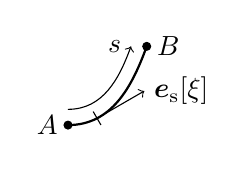
\begin{tikzpicture}
  \draw[thick] (0,0) to[out=0,in=250] coordinate[near start] (m) node[at start,left] {$A$} node[at end,right] {$B$} (1,1) ;
  \draw[->] (0,0.2) to[out=0,in=250] node[at end,left] {$s$} (0.8,1);
  \draw[|->] (m) -- +(30:0.7) node[at end,right] {$\ta e_\surf[\xi]$};
  \draw[fill,black] (0,0) circle (0.05) (1,1) circle (0.05);
 \end{tikzpicture}
 \caption{Geometry and coordinate system for 2D (and axisymmetric)}
 \label{fig:extruded}
\end{figure}

The geometry is parameterized as
\begin{align}
 \ta x &= \sum_{i=1}^n N_i[\xi]\ta x_i
  = \um N \cdot \uv X
  = \underbrace{\begin{bmatrix}N_1 & 0 & \cdots\\ 0 & N_1 & \cdots \end{bmatrix}}_{2\times 2n}\cdot \underbrace{\begin{bmatrix}x_1\\y_1\\x_2\\y_2\\ \vdots\end{bmatrix}}_{2n\times 1}
\end{align}
so the divergence and integral can be rewritten by obtaining
\begin{gather}
 J \defeq \dderiv{s}{\xi} = \norm{\ta x'}\\
 \ta e_\surf \defeq \ta x' J^{-1} = J^{-1}\sum_{i=1}^n N_i'[\xi] \ta x_i\\
 \dif A = t \dif s = t J \dif \xi     \label{eq:intdA_2d}\\
 \diff_\surf = \pderiv{}{s}\ta e_\surf = \pderiv{}{\xi}\ta e_\surf J^{-1}    \label{eq:nabla_surf_2d}
\end{gather}
and for the tangent the following derivations are also useful
\begin{align}
 \pderiv{\ta x'}{\ta x_i} &= N_i' \ts I & \pderiv{\ta x'}{\uv X} &= \um N'\\
 \pderiv{J}{\ta x_i} &= \ta e_\surf \cdot \pderiv{\ta x'}{\ta x_i} = \ta e_\surf N_i'  & \pderiv{J}{\uv X} &= \ta e_\surf\cdot \um N' \\
 \pderiv{\ta e_\surf}{\ta x_i} &= (\ts I - \ta e_\surf\otimes\ta e_\surf)N_i' J^{-1} &  \pderiv{\ta e_\surf}{\uv X} &= (\ts I - \ta e_\surf\otimes \ta e_\surf)\cdot \um N' J^{-1}
\end{align}

Plugging \eqref{eq:intdA_2d} and \eqref{eq:nabla_surf_2d} into the integral in \eqref{eq:curvature}
\begin{align}
 \int_\Omega\diff_\surf\cdot\ta w\dif A &= t \int_{-1}^{1} \ta w'\cdot \ta e_\surf \dif\xi = \left( t \int_{-1}^1 \dderiv{\ta w}{s} \cdot \ta e_\surf\dif s\right)
\end{align}
and its tangent
\begin{align}
 \int_\Omega\diff_\surf\cdot\ta w\dif A \otimes \pderiv{}{\uv X}
 =&t \int_{-1}^{1} \left(\ta w'\cdot \ta e_\surf\right)\otimes \pderiv{}{\uv X}  \dif\xi\\
 =&t \int_{-1}^{1} \ta w'\cdot \pderiv{\ta e_\surf}{\uv X} \dif\xi\\
 =&t \int_{-1}^{1} \ta w'\cdot \left(\ts I-\ta e_\surf'\otimes\ta e_\surf' \right)\cdot \um N' J^{-1} \dif\xi
\end{align}

% The boundary term is trivial
% \begin{gather}
%  \ta m = \sign[\xi]\ta e_\surf\\
%  \int_{\partial\Omega} \ta w\cdot \ta m\dif S = \ta w \cdot\ta m t = \sign[\xi]\ta w \cdot \ta e_\surf t
% \end{gather}
% and its tangent
% \begin{align}
%  \int_{\partial\Omega} \ta w\cdot \ta m\dif S\otimes \pderiv{}{\uv X} &= t \ta w\cdot\pderiv{\ta m}{\uv X}\\
%  &= \sign[\xi]t \ta w\cdot\pderiv{\ta e_\surf}{\uv X}\\
%  &= \sign[\xi]t \ta w\cdot \left(\ts I-\ta e_\surf\otimes\ta e_\surf\right)\cdot \um N' J^{-1}
% \end{align}

The load vector becomes
\begin{align}
 \uv F &= -\gamma t \int_{-1}^{1} {\um N}'^\T\cdot \ta e_\surf \dif\xi\\
       &= -\gamma t \int_{-1}^{1} \dderiv{{\um N}^\T}{s}\cdot \ta e_\surf J \dif\xi \\
 \um K &= \gamma t \int_{-1}^{1} {\um N}'^\T\cdot \left(\ts I-\ta e_\surf\otimes\ta e_\surf\right)\cdot{\um N}' J^{-1} \dif\xi\\
       &=  \gamma t \int_{-1}^{1} \dderiv{\um N^\T}{s}\cdot \left(\ts I-\ta e_\surf\otimes\ta e_\surf\right)\cdot\dderiv{\um N}{s} J \dif\xi
\end{align}
% and the boundary term
% \begin{gather}
%  \uv F = \sign[\xi]\gamma t {\um N}^\T\cdot\ta e_\surf\\
%  \um K = -\sign[\xi]\gamma t J^{-1} {\um N}^\T \cdot (\ts I - \ta e_\surf\otimes \ta e_\surf)\cdot {\um N}'
% \end{gather}

\subsection{Linear elements}
\begin{gather}
 \uv F_\linear = \gamma t L^{-1} \begin{bmatrix}x_2-x_1\\y_2-y_1\\x_1-x_2\\y_1-y_2\end{bmatrix}\\
 \um K_\linear = \gamma t L^{-1}\left(
	\begin{bmatrix}1&0&-1&0\\0&1&0&-1\\-1&0&1&0\\0&-1&0&1\end{bmatrix}-
	L^{-2}\begin{bmatrix}x_2-x_1\\y_2-y_1\\x_1-x_2\\y_1-y_2\end{bmatrix}\otimes\begin{bmatrix}x_2-x_1\\y_2-y_1\\x_1-x_2\\y_1-y_2\end{bmatrix}
  \right)
\end{gather}
% and for the boundary (boundary at $\ta x_1$)
% \begin{gather}
%  \uv F_\linear = -\gamma t L^{-1} \begin{bmatrix}x_2-x_1\\y_2-y_1\\0\\0\end{bmatrix}\\
%  \um K_\linear = -\gamma t L^{-1} \left(\begin{bmatrix}1&0&-1&0\\0&1&0&-1\\0&0&0&0\\0&0&0&0\end{bmatrix} - L^{-2} \begin{bmatrix}x_2-x_1\\y_2-y_1\\0\\0\end{bmatrix}\otimes\begin{bmatrix}x_2-x_1\\y_2-y_1\\x_1-x_2\\y_2-y_1\end{bmatrix}2\right)\\
% \end{gather}

\section{Axisymmetric}
For brevity, the notation $(\bullet)' = \pderiv{\bullet}{\xi}$ or $(\bullet)' = \pderiv{\bullet}{\theta}$ is used for $f[\xi]$ and $f[\theta]$ respectively.

This part was more complicated than initially estimated.
I have consistently decomposed variables into $\ts Q$ to make this managable and also analytically calculating the integral over $\theta$.

With cylindrical coordinates $\ta r = r\ta e_r + z \ta e_z$.
\begin{align}
 \ta r &= \sum_i N_i[\xi]\ta r_i = \um N\cdot \uv R\\
 x &= \cos[\theta] r\\
 y &= \sin[\theta] r\\
 z &= z\\
 \ts Q &= \begin{bmatrix}\cos[\theta] & 0\\ \sin[\theta] & 0\\ 0 & 1\end{bmatrix}\\
 \ta x &= \ts Q[\theta] \cdot \ta r[\xi]\\
 \ta w &= \ts Q[\theta] \cdot \ta v[\xi]\\
 \ta m &= \ts Q[\theta] \cdot \ta t[\xi]
\end{align}

Since we have a convenient orthogonality, we can treat $\xi$ and $\theta$ seperarely.
\begin{align}
 J_\xi &= \norm{\pderiv{\ta x}{\xi}} = \norm{\ts Q \cdot \ta r'} = \norm{\ta r'}\\
 J_\theta &= \norm{\pderiv{\ta x}{\theta}} = \norm{\ts Q' \cdot \ta r} = r \\
 \dif A &= J_\xi J_\theta \dif \xi \dif \theta \\
 \diff_\surf &= J_\xi^{-2} \pderiv{\ta x}{\xi}\pderiv{}{\xi} + J_\theta^{-2} \pderiv{\ta x}{\theta}\pderiv{}{\theta}
\end{align}
and for the tangent the following derivations are also usefull
\begin{align}
 \ta e_\surf &\defeq \ta r' J_\xi^{-1} & \uv D &\defeq \um N^\T \cdot \ta e_\surf\\
 \uv A &\defeq {\um N}'^\T \cdot \ta e_\surf & \uv B &\defeq \pderiv{r}{\uv R} = {\um N}^\T \cdot \begin{bmatrix}1\\0\end{bmatrix}\\
\end{align}
\begin{align}
 \pderiv{\ta r'}{\ta r_i} &= N_i' \ts I
	& \pderiv{\ta r'}{\uv R} &= \um N'\\
 \pderiv{J_\xi}{\ta r_i} &= \ta e_\surf \cdot \pderiv{\ta r'}{\ta r_i} = \ta e_\surf N_i'
	& \pderiv{J_\xi}{\uv R} &= \ta e_\surf\cdot \um N' \\
 \pderiv{\ta e_\surf}{\ta r_i} &= (\ts I - \ta e_\surf\otimes\ta e_\surf)N_i' J_\xi^{-1}
	& \pderiv{\ta e_\surf}{\uv R} &= (\ts I - \ta e_\surf \otimes \ta e_\surf )\cdot \um N' J_\xi^{-1}
\end{align}

Plugging this into \eqref{eq:curvature} to obtain
\begin{align}
 &\int_\Omega\diff_\surf\cdot\ta w\dif A\\
=&\int_{-1}^{1}\int_0^{2\pi}\left( J_\xi^{-2} \pderiv{\ta x}{\xi}\cdot\pderiv{\ta w}{\xi} +
                              J_\theta^{-2} \pderiv{\ta x}{\theta}\cdot\pderiv{\ta w}{\theta}
  \right) J_\xi J_\theta \dif \theta \dif \xi\\
=&\int_{-1}^{1}\int_0^{2\pi}\left(
	  J_\xi^{-2} (\ts Q^\T\cdot\ts Q):(\ta r'\otimes \ta v') +
	  J_\theta^{-2} ({\ts Q'}^\T\cdot\ts Q'):(\ta r\otimes\ta v)
  \right) J_\xi J_\theta \dif \theta \dif \xi\\
=&\int_{-1}^{1}\int_0^{2\pi}\left(
	  J_\xi^{-2} \ts I :(\ta r'\otimes \ta v') +
	  J_\theta^{-2} \begin{bmatrix}1&0\\0&0\end{bmatrix}:(\ta r \otimes \ta v)
  \right) J_\xi J_\theta \dif \theta \dif \xi\\
=&2\pi\int_{-1}^{1}\left( \ta v' \cdot \ta e_\surf r + \ta v \cdot \begin{bmatrix}1\\0\end{bmatrix} J_\xi \right) \dif \xi\\
=&2\pi\int_{-1}^{1}\left( \dderiv{\ta v}{s} \cdot \ta e_\surf r + \ta v \cdot \begin{bmatrix}1\\0\end{bmatrix} \right) \dif s
\end{align}
and its tangent
\begin{align}
 &\int_\Omega\diff_\surf\cdot\ta w\dif A \otimes \pderiv{}{\uv R} \\
 =& 2\pi \int_{-1}^{1} \left(
	\ta v' \cdot \ta e_\surf r + \ta v\cdot \begin{bmatrix}1\\0\end{bmatrix} J_\xi
	\right)\otimes\pderiv{}{\uv R}\dif\xi\\
  =& 2\pi \int_{-1}^{1} \left(
	\ta v' \cdot \ta e_\surf \otimes \pderiv{r}{\uv R} + \ta v'\cdot \pderiv{\ta e_\surf}{\uv R} r + \ta v\cdot \begin{bmatrix}1\\0\end{bmatrix}\otimes\pderiv{J_\xi}{\uv R}
	\right)\dif\xi\\
  =& 2\pi \int_{-1}^{1} \bigg(
	\ta v' \cdot \ta e_\surf \otimes\left(\begin{bmatrix}1&0\end{bmatrix}\cdot \um N\right) +
	\ta v'\cdot (\ts I - \ta e_\surf\otimes \ta e_\surf)\cdot \um N' J_\xi^{-1} r
	+\ta v\cdot \begin{bmatrix}1\\0\end{bmatrix}\otimes (\ta e_\surf\cdot \um N')
	\bigg)\dif\xi
\end{align}

% The boundary term is computed as
% \begin{align}
%  \int_{\partial\Omega} \ta w\cdot\ta m\dif S &= \int_0^{2\pi} (\ts Q^\T\cdot \ts Q):(\ta v\cdot\ta t) r \dif \theta\\
%   &= 2\pi r \ta v \cdot \ta t = 2\pi\sign[\xi]r \ta v\cdot \ta e_\surf
% \end{align}
% and its tangent
% \begin{align}
%  \int_{\partial\Omega} \ta w\cdot\ta m\dif S \otimes \pderiv{}{\uv R} &= 2\pi\sign[\xi] (r \ta v \cdot \ta e_\surf)\otimes \pderiv{}{\uv R}\\
%   &= 2 \pi \sign[\xi]\left(\ta v\cdot\ta e_\surf\otimes\pderiv{r}{\uv R} + r \ta v\cdot\pderiv{\ta t}{\uv R}\right)\\
%   &= 2 \pi \sign[\xi]\left(\ta v\cdot\ta e_\surf\otimes\left(\begin{bmatrix}1&0\end{bmatrix}\cdot\um N\right) +  J_\xi^{-1} r \ta v\cdot\left(\ts I-\ta e_\surf\otimes\ta e_\surf\right)\cdot \um N'\right)
% \end{align}

The load vector for an element is
\begin{gather}
 \uv F = -2\pi \gamma \int_{-1}^{1} \left(r{\um N}'^\T\cdot\ta e_\surf + J_\xi{\um N}^\T\cdot\begin{bmatrix}1\\0\end{bmatrix}\right) \dif\xi
\end{gather}
\begin{multline}
 \um K = 2\pi \int_{-1}^{1} \bigg(
	{\um N}'^\T \cdot \ta e_\surf \otimes {\um N}^\T\cdot \begin{bmatrix}1\\0\end{bmatrix} +\\
	{\um N}'^\T \cdot (\ts I - \ta e_\surf\otimes \ta e_\surf)\cdot {\um N}' J_\xi^{-1} r +
	{\um N}^\T \cdot \begin{bmatrix}1\\0\end{bmatrix}\otimes \ta e_\surf\cdot {\um N}'
	\bigg)\dif\xi
\end{multline}
or
\begin{gather}
  \uv F = -2\pi \gamma \int_{-1}^{1} \left(r\uv A + J_\xi\uv B\right) \dif\xi\\
  \um K = 2\pi \int_{-1}^{1} \bigg(
	\uv A \otimes \uv B +
	\uv B\otimes \uv A +
	J_\xi^{-1} r({\um N}'^\T \cdot {\um N}' - \uv A\otimes \uv A)
	\bigg)\dif\xi
\end{gather}
% and for the boundary
% \begin{align}
%  \uv F &= 2\pi\gamma\sign[\xi] r {\uv N}^\T \cdot \ta e_\surf = 2\pi\gamma\sign[\xi]\uv D\\
%  \um K &= -2 \pi \gamma \sign[\xi]\um N^\T\cdot\left(\ta e_\surf\otimes\left(\um N^\T\cdot\begin{bmatrix}1\\0\end{bmatrix}\right) + J_\xi^{-1} r \left(\ts I-\ta e_\surf\otimes\ta e_\surf\right)\cdot \um N' \right)\\
%        &= -2 \pi \gamma \sign[\xi]\left(\uv D\otimes\uv B + J_\xi^{-1} r \left(\um N^\T\cdot\um N' -\uv D\otimes\uv A\right) \right)
% \end{align}

\subsection{Linear elements}

\begin{gather}
 \nonumber \hat{\uv A} = -L^{-1}\begin{bmatrix}r_2-r_1\\z_2-z_1\\r_1-r_2\\z_1-z_2\end{bmatrix}, \quad
 \hat{\uv B} = \begin{bmatrix}1\\0\\1\\0\end{bmatrix},\quad J_\xi = \frac12 L\\
 \uv F_\linear = -\pi \gamma \left((r_1+r_2)\hat{\uv A} + L\hat{\uv B}\right)\\
 \um K_\linear = \pi \gamma \left(
  \hat{\uv A}\otimes\uv B + \hat{\uv B}\otimes\hat{\uv A}
  + 2L^{-1} r \left(\begin{bmatrix}1&0&-1&0\\0&1&0&-1\\-1&0&1&0\\0&-1&0&1\end{bmatrix} - \hat{\uv A}\otimes\hat{\uv A}\right)
  \right)
\end{gather}
% and for boundary at $\ta r_1$;
% \begin{gather}
%  \nonumber \uv B = \begin{bmatrix}1\\0\\0\\0\end{bmatrix}, \quad \uv D = L^{-1}\begin{bmatrix}r_2-r_1\\z_2-z_1\\0\\0\end{bmatrix}\\
%  \uv K_\linear = 2\pi \gamma\left(\uv D\otimes \uv B + L^{-1} r_1 \left(\begin{bmatrix}-1&0&1&0\\0&-1&0&1\\0&0&0&0\\0&0&0&0\end{bmatrix}- \uv D\otimes \hat{\uv A}\right)\right)\\
%  \uv F_\linear = -2\pi \gamma r_1 L^{-1} \begin{bmatrix}r_2-r_1\\z_2-z_1\\0\\0\end{bmatrix}
% \end{gather}

\newpage
\section{General 3D}

Introducing another parameter $\zeta$ in order to obtain a nice mapping.
\begin{align}
 \ta x[\xi,\eta,\zeta] &= (1+\zeta)\ta n + \sum_i N_i[\xi,\eta]\ta x_i  %= \ta n + \um N \cdot \uv X\\
  %&= (1-\zeta) \begin{bmatrix}N_1 & 0 & 0 & N_2 & \cdots\\0&N_1&0&0&\cdots\\0&0&N_1&0&\cdots\end{bmatrix}\cdot\begin{bmatrix}x_1\\y_1\\z_1\\x_2\\\vdots\end{bmatrix}
\end{align}

\begin{gather}
 J \defeq \norm{\pderiv{\ta x}{\xi} \times  \pderiv{\ta x}{\eta}}\\
 \ta n = \pderiv{\ta x}{\xi} \times \pderiv{\ta x}{\eta} J^{-1}\\
 \begin{bmatrix}\dif x\\ \dif y\\ \dif z\end{bmatrix} =
  \underbrace{\begin{bmatrix}\pderiv{x}{\xi} & \pderiv{x}{\eta} & \pderiv{x}{\zeta}\\
	  \pderiv{y}{\xi} & \pderiv{y}{\eta} & \pderiv{y}{\zeta}\\
	  \pderiv{z}{\xi} & \pderiv{z}{\eta} & \pderiv{z}{\zeta} \end{bmatrix}}_{\ts J}
  \cdot \begin{bmatrix}\dif \xi \\ \dif \eta \\ \dif \zeta\end{bmatrix}\\
  \ts J = \begin{bmatrix}\pderiv{x}{\xi} & \pderiv{x}{\eta} & n_1\\
	  \pderiv{y}{\xi} & \pderiv{y}{\eta} & n_2\\
	  \pderiv{z}{\xi} & \pderiv{z}{\eta} & n_3 \end{bmatrix}\\
 \diff = \ts J^{-\T}\cdot\diff_\xi\\
 \dif A = J \dif \xi \dif \eta 
\end{gather}

and we obtain
\begin{align}
 &\iint_\Omega\diff_\surf\cdot\ta w\dif A\\
=&\iint_\omega(\ts I-\ta n\otimes\ta n):(\ta w\otimes \ts J^{-\T}\cdot\diff_\xi)J\dif\xi\dif\eta\big|_{\zeta=0}\\
=&\iint_\omega(\ts I-\ta n\otimes\ta n):\left((\ta w\otimes\diff_\xi) \cdot\ts J^{-1}\right)J\dif\xi\dif\eta\big|_{\zeta=0}
%=&\iint_\omega((\ts I-\ta n\otimes\ta n)\cdot\ts J^{-\T}):(\ta w\otimes\diff_\xi)J\dif\xi\dif\eta\big|_{\zeta=0}\\
%=&\iint_\omega(\ta w\otimes\diff_\xi):((\ts I-\ta n\otimes\ta n)\cdot\ts J^{-\T})J\dif\xi\dif\eta\big|_{\zeta=0}
\end{align}

% And given an edge along $\xi$;
% \begin{align}
%  &\int_{\partial\Omega}\ta w\cdot\ta m\dif S\\
% =&\int_{\partial\omega}\ta w\cdot\ta m J_\xi \dif \xi\\
%  \hat{\ta n} &= \ta e_\xi \times \ta e_\eta\\
%  \hat{\ta m} &= \ta e_\xi \times \hat{\ta n} = \ta e_\xi\times (\ta e_\xi \times \ta e_\eta)\\
%  \ta m &= \hat{\ta m}\norm{\ta m}^{-1}
% \end{align}

It becomes a bit tricky to express the load vector nicely due to the appearance of a third order tensor, it will need to be reshaped.
After some rewriting the expression becomes
\begin{align}
 \hat{\uv N} &= \begin{bmatrix} N_1\\ N_2\\ \vdots\end{bmatrix}\\
 \hat{\um B} &= \ts J^{-\T}\cdot(\diff_\xi\cdot(\hat{\uv N})^\T)\\
 \hat{\um F} &= \iint_\omega(\ts I-\ta n \cdot \ta n^\T)\cdot \hat{\um B} J\dif\xi\dif\eta\big|_{\zeta=0}\\
 \uv F &= \begin{bmatrix}\hat{\uv F}_{1:}\\\hat{\uv F}_{2:}\\\vdots\end{bmatrix}
\end{align}
% and along the boundary
% \begin{align}
%  \uv F &= \int_{\partial\omega}{\um N}^\T\cdot\ta m J_\xi \dif \xi
% \end{align}

\newpage
\section{General 3D alternative method}
\begin{align}
 \ta x[\xi,\eta] = \sum_i N_i[\xi,\eta]\ta x_i
\end{align}
\begin{gather}
 J \defeq \norm{\pderiv{\ta x}{\xi} \times  \pderiv{\ta x}{\eta}}\\
 \ta n = \pderiv{\ta x}{\xi} \times \pderiv{\ta x}{\eta} J^{-1}\\
 \ta e_\surf = \pderiv{\ta x}{\xi}\norm{\pderiv{\ta x}{\xi}}^{-1}\\
 \ta e_\tangent = -\ta e_\surf\times \ta n\\
 \begin{bmatrix}\dif x\\ \dif y\\ \dif z\end{bmatrix} =
  \underbrace{\begin{bmatrix}\pderiv{\ta x}{\xi} & \pderiv{\ta x}{\eta}
  \end{bmatrix}}_{\ts J''}
  \cdot \begin{bmatrix}\dif \xi \\ \dif \eta\end{bmatrix}\\
 \begin{bmatrix}\dif s\\ \dif t\end{bmatrix} =
  \underbrace{\begin{bmatrix} \ta e_\surf^\T \\ \ta e_\tangent^\T
  \end{bmatrix}}_{\ts J'}
  \cdot \begin{bmatrix}\dif x \\ \dif y \\ \dif z\end{bmatrix}\\
 \dif A = J \dif \xi \dif \eta
\end{gather}

\begin{align}
 \diff_\surf\cdot\ta w &= \diff_{st}\cdot\ta w_{st} \\
 &= (\ta w_{st}\otimes\diff_{st}):\ts I \\
 &= \left(((\ts J'\cdot \ta w) \otimes \diff_{\xi\eta})\cdot \left(\ts J'\cdot\ts J''\right)^{-1}\right): \ts I\\
 &= \left((\ta w\cdot (\ts J'^\T \otimes \diff_{\xi\eta}) +\ts J'\cdot(\ta w\otimes\diff_{\xi\eta}) )\cdot \left(\ts J'\cdot\ts J''\right)^{-1}\right): \ts I
\end{align}
The gradient $\ts J'^\T \otimes\diff_{\xi\eta}$ is bothersome.
\begin{align}
 \ta e_\surf \otimes \diff_{\xi\eta} = \text{ugh...}
\end{align}

Considering the special case of linear surfaces;
\begin{align}
  \diff_\surf\cdot\ta w &= \left(\ts J'\cdot(\ta w\otimes\diff_{\xi\eta})\cdot \left(\ts J'\cdot\ts J''\right)^{-1}\right): \ts I
\end{align}

\begin{align}
 &\iint_\Omega\diff_\surf\cdot\ta w\dif A\\
=&\iint_\omega \ts I:\left(\ts J'\cdot(\ta w\otimes\diff_{\xi\eta})\cdot \left(\ts J'\cdot\ts J''\right)^{-1}\right)J\dif\xi\dif\eta
\end{align}


\newpage
\section{General 3D alternative 2}
\begin{align}
 \ta w \cdot \ts\nabla_{s} = (\ta w \otimes \diff) : (\ts I - \ta n \otimes \ta n)= (\ta w \otimes \diff)^\sym : (\ts I - \ta n \otimes \ta n)
\end{align}
FE implementation
\begin{align}
 \uv F = \um{B}^\T \cdot \begin{pmatrix} 1 - n_1 n_1 \\ 1 - n_2 n_2 \\ 1 - n_3 n_3 \\ -n_2 n_3 \\ -n_1 n_3 \\ -n_1 n_2 \end{pmatrix}
\end{align}


\begin{gather}
 J \defeq \norm{\pderiv{\ta x}{\xi} \times  \pderiv{\ta x}{\eta}}\\
 \ta n = \pderiv{\ta x}{\xi} \times \pderiv{\ta x}{\eta} J^{-1}\\
 \dif A = J \dif a
\end{gather}

\begin{align}
 \int_\Omega \ta w\cdot\diff_\surf \dif A \to \int_\omega \uv F J \dif a
\end{align}



\end{document}
